\documentclass[../main.tex]{subfiles}
\graphicspath{{\subfix{../figures/}}}
%
\begin{document}
\section{简单工厂模式}
设计模式是一套解决软件开发过程中某些常见问题的通用解决方案,是已被反复使用且证明其有效性的设计经验的总结。
目的是建立具有可复用、可维护、可扩展的软件系统。
\begin{itemize}
  \item \textbf{创建型模式},共5种:工厂方法模式、抽象工厂模式、单例模式、建造者模式、原型模式。
  \item \textbf{结构型模式},共7种:适配器模式、装饰模式、代理模式、外观模式、桥接模式、组合模式、享元模式。
  \item \textbf{行为型模式},共11种:策略模式、模板方法模式、观察者模式、迭代子模式、责任链模式、命令模式、备忘录模式、状态模式、访问者模式、中介者模式、解释器模式。
\end{itemize}
\textbf{创建型的设计模式}:创建模式是对类的实例化过程的抽象。一些系统在创建对象时,需要动态地决定怎样创建对象,创建哪些对象,以及如何组合和表示这些对象,实现对象的``创建''与``使用''相分离。

\textbf{简单工厂模式}:
\begin{itemize}
  \item 简单工厂模式又叫做静态工厂方法(Static Factory Method)模式。
  \item 简单工厂模式是由一个工厂对象决定创建出哪一种产品类的实例。
k \item 工厂模式专门负责将大量有共同接口的类实例化。工厂模式可以动态决定将哪一个类实例化,不必事先知道每次要实例化哪一个类。
\end{itemize}
\begin{lstlisting}[language=java]
class 消费者 {
  public void 消费() {
    鼠标 obj1 = 工厂.生产(“鼠标”);
    铅笔 obj2 = 工厂.生产(“铅笔”);
    // ...
  }
}
\end{lstlisting}
%
\subsection{简单工厂模式的引进}
\noindent 比如说有一个生产水果的农场,专门向市场销售各类水果。在这个系统里需要描述下列的水果:
\begin{itemize}
  \item 葡萄 Grape
  \item 草莓 Strawberry
  \item 苹果 Apple
\end{itemize}
\begin{figure}[H]
  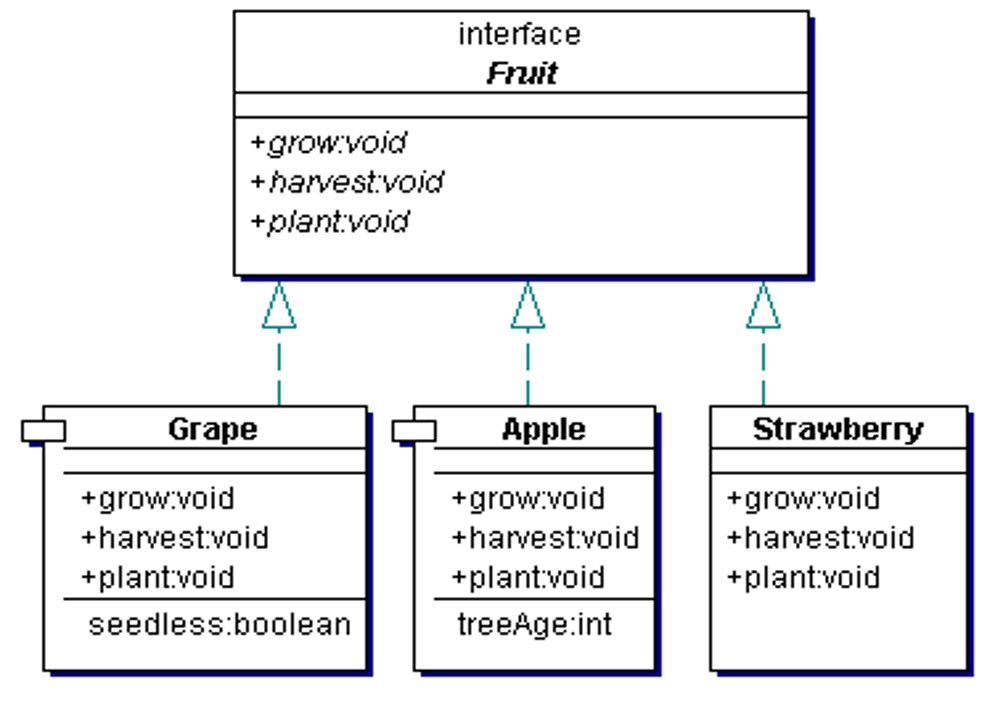
\includegraphics[width=0.40\textwidth]{15_1.jpg}
\end{figure}
\begin{lstlisting}[language=java]
public interface Fruit {
  void grow(); // 生长
  void harvest(); // 收获
  void plant(); //种植
}
\end{lstlisting}
\begin{lstlisting}[language=java]
public class Apple implements Fruit {
  private int treeAge;
  // 生长
  public void grow() { System.out.println("Apple is growing"); }
  // 收获
  public void harvest() { System.out.println("Apple has been harvested"); }
  // 种植
  public void plant() { System.out.println("Apple has been planted"); }
  // 树龄的取值方法
  public int getTreeAge() { return treeAge; }
  // 树龄的赋值方法
  public void setTreeAge(int treeAge) { this.treeAge = treeAge; }
}
\end{lstlisting}
\begin{lstlisting}[language=java]
public class Grape implements Fruit {
  private boolean seedless;
  // 生长
  public void grow() { System.out.println ("Grape is growing"); }
  // 收获
  public void harvest() { System.out.println("Grape has been harvested"); }
  // 种植
  public void plant() { System.out.println("Grape has been planted"); }
  // 有无籽的取值方法
  public boolean getSeedless() { return seedless; }
  // 有无籽的赋值方法
  public void setSeedless(boolean seedless) { this.seedless = seedless; }
}
\end{lstlisting}
\begin{lstlisting}[language=java]
public class Strawberry implements Fruit {
  public void grow() {
    System.out.println("Strawberry is growing");
  }
  public void harvest() {
    System.out.println("Strawberry has been harvested");
  }
  public void plant() {
    System.out.println("Strawberry has been planted");
  }
}
\end{lstlisting}
农场的园丁也是系统的一部分,由FruitGardener 类代表。其结构由下面的类图描述。
FruitGardener 类会根据客户端的要求,创建出不同的水果对象,比如苹果(Apple),葡萄(Grape)或草莓(Strawberry)的实例。
\begin{lstlisting}[language=java]
public class FruitGardener {
  // 静态工厂方法
  public static Fruit factory(String which)
  throws BadFruitException {
    if (which.equalsIgnoreCase("apple")) {
      return new Apple();
    } else if (which.equalsIgnoreCase("strawberry")) {
      return new Strawberry();
    } else if (which.equalsIgnoreCase("grape")) {
      return new Grape();
    } else {
      throw new BadFruitException("Bad fruit request");
    }
  }
}

class BadFruitException extends Exception {
  public BadFruitException(String msg) {
    super(msg);
  }
}
\end{lstlisting}
可以看出,园丁类提供了一个静态工厂方法。在客户端的调用下,这个方法创建客户端所需要的水果对象。
如果客户端的请求是系统所不支持的,工厂方法就会抛出一个BadFruitException 异常。
在使用时,客户端只需调用FruitGardener 的静态方法factory()即可。
\begin{lstlisting}[language=java]
try {
  FruitGardener.factory("grape");
  FruitGardener.factory("apple");
  FruitGardener.factory("strawberry");
  // ...
} catch(BadFruitException e) {
  // ...
}
\end{lstlisting}
%
\subsection{简单工厂模式的结构}
简单工厂模式是类的创建模式,这个模式的一般性结构如下图所示。
\begin{figure}[H]
  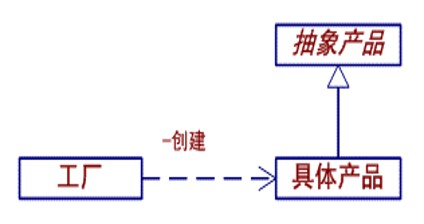
\includegraphics[width=0.30\textwidth]{15_2.jpg}
\end{figure}
\textbf{角色与结构}:简单工厂模式就是由一个工厂类可以根据传入的参数决定创建出哪一种产品类的实例。下图所示为以一个示意性的实现为例说明简单工厂模式的结构。
\begin{figure}[H]
  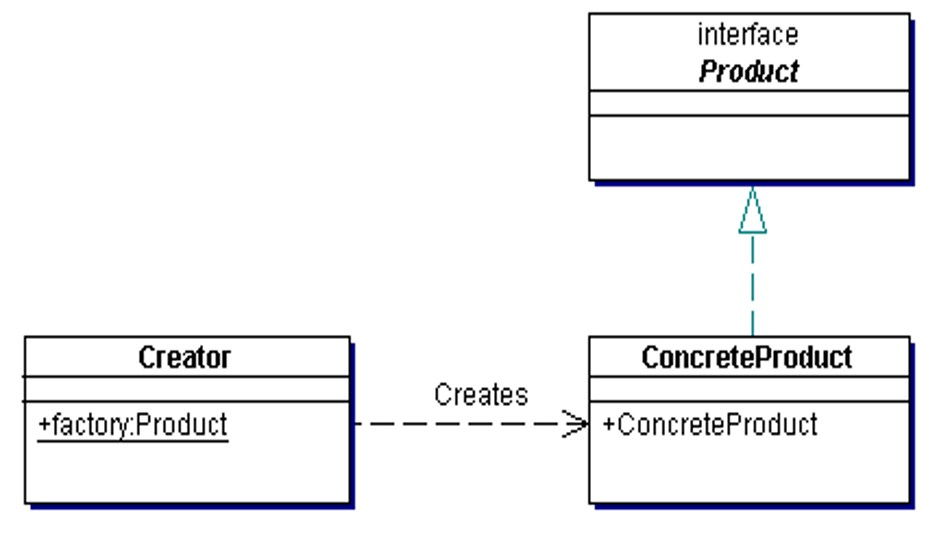
\includegraphics[width=0.45\textwidth]{15_3.jpg}
\end{figure}
%
\noindent 从上图可看出,简单工厂模式涉及到工厂角色、抽象产品角色及具体产品角色三个角色:
%
\begin{itemize}
  \item 工厂类(Creator)角色:担任这个角色的是工厂方法模式的核心,含有与应用紧密相关的业务逻辑。工厂类在客户端的直接调用下创建产品对象,它往往由一个具体Java 类实现。
  \item 抽象产品(Product)角色:担任这个角色的类是工厂方法模式所创建的对象的父类,或它们共同拥有的接口。抽象产品角色可以用一个Java 接口或者Java 抽象类实现。
  \item 具体产品(Concrete Product)角色:工厂方法模式所创建的任何对象都是这个角色的实例,具体产品角色由一个具体Java 类实现。
\end{itemize}
抽象产品角色的主要目的是给所有的具体产品类提供一个共同的类型,在最简单的情况下,可以简化为一个标识接口。
%
\begin{lstlisting}[language=java]
public class Creator {
  // 静态工厂方法
  public static Product factory() {
    return new ConcreteProduct();
  }
}
public interface Product {  }
public class ConcreteProduct implements Product {
  public ConcreteProduct() {  }
}
\end{lstlisting}
如果系统仅有一个具体产品角色的话,那么就可以省略掉抽象产品角色。
%
\subsection{简单工厂模式的实现}
\noindent \textbf{多层次的产品结构}:在实际应用中,产品可以形成复杂的等级结构.这个时候,简单工厂模式采取的是以不变应万变的策略,一律使用同一个工厂类。如下图所示。图中从Factory 类到各个Product 类的虚线代表创建(依赖)关系;从Client 到其他类的联线是一般依赖关系。
%
\begin{figure}[H]
  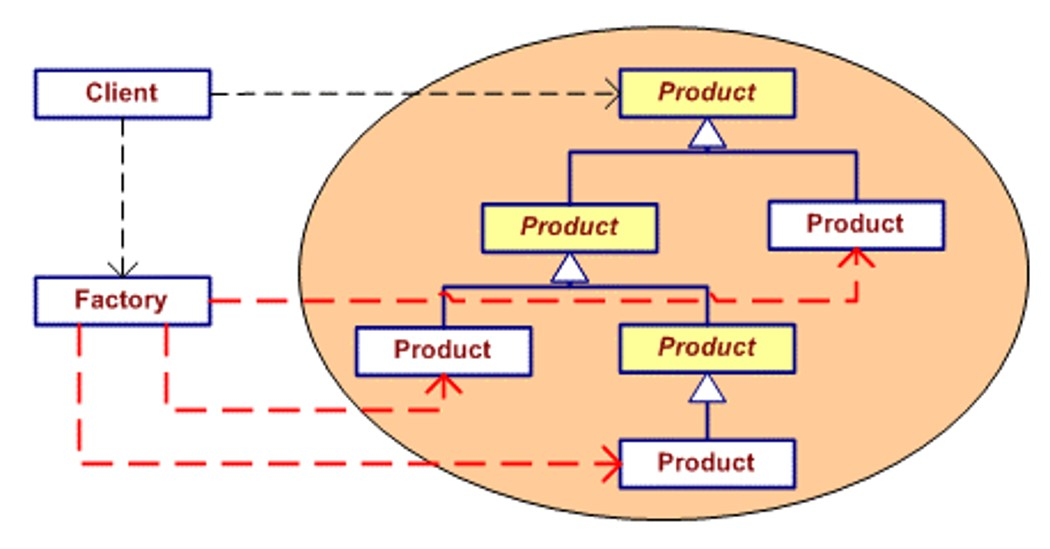
\includegraphics[width=0.45\textwidth]{15_4.jpg}
\end{figure}
%
这样做的好处是设计简单,产品类的等级结构不会反映到工厂类中来。但是这样做的缺点是,
增加新的产品必将导致工厂类的修改.

\textbf{使用Java 接口或者Java 抽象类}:
\begin{itemize}
  \item 如果具体产品类彼此之间没有共同的业务逻辑,那么抽象产品角色可以由一个Java 接口扮演;
  \item 相反,如果这些具体产品类彼此之间确有共同的业务逻辑,那么这些公有的逻辑就应当移到抽象角色里面,这就意味着抽象角色应当由一个抽象类扮演。在一个类型的等级结构里面,共同的代码应当尽量向上移动,以达到共享的目的,如下图所示。
\end{itemize}
\textbf{工厂角色与抽象产品角色合并}:在有些情况下, 工厂角色可以由抽象产品角色扮演。典型的应用就是java.text.DateFormat 类,一个抽象产品类同时是子类的工厂.
\begin{lstlisting}[language=java]
Date date = new Date();
//日期格式,精确到日 2017-4-16
DateFormat df1 = DateFormat.getDateInstance();
System.out.println(df1.format(date));

 //可以精确到秒 2017-4-16 12:43:37
DateFormat df2 = DateFormat.getDateTimeInstance();
System.out.println(df2.format(date));

//只显示出时时分秒 12:43:37
DateFormat df3 = DateFormat.getTimeInstance();
System.out.println(df3.format(date));
\end{lstlisting}
\textbf{三个角色全部合并}:如果抽象产品角色已经被省略,而工厂角色就可以与具体产品角色合并。换言之,一个产品类为创建自身的工厂.
显然,三个原本独立的角色:工厂角色、抽象产品以及具体产品角色都已经合并成为一个类,这个类自行创建自己的实例。
\begin{lstlisting}[language=java]
public class ConcreteProduct {
  public ConcreteProduct() {  }
  // 静态工厂方法
  public static ConcreteProduct factory() {
    return new ConcreteProduct();
  }
}
\end{lstlisting}
这种退化的简单工厂模式与单例模式以及多例模式有相似之处,但是并不等于单例或者多例模式。

\textbf{产品对象的循环使用和登记式的工厂方法}:在很多情况下,产品对象可以循环使用。换言之,工厂方法可以循环使用已经创建出来的对象,而不是每一次都创建新的产品对象。
如果工厂方法总是循环使用同一个产品对象,那么这个工厂对象可以使用一个属性来存储这个产品对象。每一次客户端调用工厂方法时,工厂方法总是提供这同一个对象。
\begin{lstlisting}[language=java]
class Factory {
  static Product obj;
  public static void factory(int type) {
    // ...
    if(obj==null)
    obj=new ConcreteProduct();
    return obj;
    // ...
  }
}
\end{lstlisting}
%
\subsection{简单工厂模式的优缺点}
\textbf{优点}:客户端则可以免除直接创建产品对象的责任,而仅仅负责消费产品。
对于消费者角色来说,任何时候需要某种产品,只需要向工厂角色(下订单)请求即可,而无需知道产品创建细节。
实现了客户端类与产品类的解耦。

\textbf{缺点}:当产品种类增加时,工厂类的工厂方法也必须随之修改。

这个工厂类集中了所有的产品创建逻辑,形成一个无所不知的全能类,有人把这种类叫做上帝类(God Class)。如果这个全能类代表的是农场的一个具体园丁的话,那么这个园丁就需要对所有的产品负责,成了农场的关键人物,他什么时候不能正常工作了, 整个农场都要受到影响。

\noindent \textbf{对开闭原则的支持}:开闭原则要求一个系统的设计能够允许系统在无需修改的情况下,扩展其功能。那么简单工厂模式是否满足这个条件?
要回答这个问题,首先需要将系统划分成不同的子系统,再考虑功能扩展对于这些子系统的要求。一般而言,一个系统总可以划分成为产品的消费者角色(Client)、产品的工厂角色(Factory)以及产品角(Product)三个子系统.
在这个系统中,功能的扩展体现在引进新的产品上。开闭原则要求系统允许当新的产品加入系统中,而无需对现有代码进行修改。这一点对于产品的消费角色是成立的,而对于工厂角色是不成立的。
简单工厂角色只在有限的程度上支持开闭原则。
\end{document}
